\documentclass[a4paper, 11pt, cn]{elegantpaper}
\usepackage{ctex}
\usepackage{amssymb}
\usepackage{array}
\usepackage{xcolor}
\usepackage{cancel}
\usepackage{color}
\usepackage{tikz}
\usepackage{minted}
\usepackage{algorithmic}
\usepackage{algorithm2e}
\usepackage{xeCJK}
\usepackage{hyperref}
\usepackage{amsmath, amsthm}
\usepackage{mathrsfs}
\usepackage{tcolorbox}
\usepackage{graphicx}
\tcbuselibrary{skins}
\tcbuselibrary{minted}
\usemintedstyle{lovelace}
\title{一次使用 Java 进行机器学习的实验尝试}
\author{禚文宇 \\ 202100800179}
\date{\today}

\begin{document}

\maketitle

\begin{abstract}
    本次实验使用了 3w 数据集,通过 KNN 算法和朴素贝叶斯算法对给定的数据集进行了分类的工作,最终前者的正确率在 $k=3$ 时可以达到 95$\%$ 以上,后者的正确率可以达到99.444$\%$。
    同时我使用了 \texttt{Python} 为训练后得到的结果进行了可视化处理,获得了一张真实分类与预测分类的对照图,以上代码及运行结果均可在我的\href{https://gitee.com/Dusker_233/sduw_-java_-ml_2022}{gitee项目}和\href{https://github.com/Dusker233/sduw_java_mltest}{github项目}中找到。
\end{abstract}

\tableofcontents
\newpage

\section{数据集介绍}
本次上机作业使用的是 3w 数据集,3w 数据集是第一个公开的记录了油井中罕见的不良真实事件的数据集,可以作为基准数据集,用于开发与实际数据固有困难相关的机器学习技术。

关于该数据集背后的理论的更多信息,可在《石油科学与工程杂志》(Journal of Petroleum Science and Engineering)上发表的论文《油井中罕见不良真实事件的现实和公共数据集》\cite{3w}中找到。

对于数据集中的数据,其部分属性信息如下表所示:

\begin{table}[htbp]\centering
    \begin{tabular}{c|c}
    \hline
    属性    & 含义         \\ \hline
    P-PDG & 永久井下压力表的压力 \\ \hline
    P-TPT & 压力传感器的数据   \\ \hline
    T-TPT & 温度传感器的数据   \\ \hline
    \end{tabular}
    \caption{数据部分属性信息}
\end{table}

\section{使用的算法介绍}

本次上机实验,我尝试了两个分类算法,分别为K-最近邻(KNN)算法和朴素贝叶斯算法,下面我将简单介绍这两个算法。

\subsection{K-最近邻算法(KNN)介绍}

K-最近邻算法(KNN)是一种用于分类和回归的非参数统计方法:
\begin{enumerate}
    \item 在 KNN-分类中,通过 $K$ 个最近邻居中出现次数最多的分类决定了此对象的分类;
    \item 在 KNN-回归中,$K$ 的最近邻居的值的平均值将会称为此对象的预测值。
\end{enumerate}

KNN 是一个非常易于理解的机器学习算法,分为计算距离、取 $K$ 个最近邻居、根据邻居分类三个步骤。

\subsubsection{具体过程}

\begin{enumerate}
    \item 计算距离:在 KNN 中,我们通过 Euclid 距离来度量两个对象 $\theta_0=\left(x_0, x_1, \cdots, x_n\right)$ 和 $\theta_1 = \left(y_0, y_1, \cdots, y_n\right)$
之间的距离,具体定义为
$$\operatorname{dis}(\theta_0, \theta_1) = \sum\limits_{i=0}^{n}\sqrt{\left(x_i - y_i\right)^2}$$

    必须注意到的是,两个对象必须具有相同的数据维度,否则 Euclid 距离将无法计算。
    \item 取 $K$ 个最近邻居:本步骤非常容易,即按照 Euclid 距离排序后,取前 $K$ 个互异的数据点即可。
    \item 在 根据邻居分类:KNN-分类中,我们只需取出这 $K$ 个最近邻居的标签,找出出现次数最多的标签即为返回值。
\end{enumerate}


\subsection{朴素贝叶斯算法介绍}

朴素贝叶斯算法是一个基于贝叶斯公式的算法:设 $(\Omega, \mathscr{F}, P)$ 是概率空间,$A_1, A_2, \dots, A_n$ 是样本空间 $\Omega$ 的一个分割,则对任意 $B \in \mathscr{F}$,$P(B) > 0$,有
$$P\left(A_k \mid B\right) = \dfrac{P(A_k)P(B \mid A_k)}{\sum\limits_{j = 1}^nP(A_j)P(B \mid A_j)}$$ 我们可以这样理解这个公式:假设某个过程具有 $A_1, A_2, \cdots, A_n$ 这样 $n$ 个可能的前提(原因),而 $P(A_1), P(A_2), \cdots, P(A_n)$ 是
人们对这 $n$ 个可能的前提(原因)的可能性大小的一种事前估计,称之为\textbf{先验概率}。当这个过程有了一个结果 $B$ 之后,人们会通过条件概率 $P(A_1 \mid B), P(A_2 \mid B), \cdots, P(A_n \mid B)$ 来对这 $n$ 个可能前提的可能性大小做出一个新的认识,
因此将这些条件概率称之为\textbf{后验概率},而贝叶斯公式恰好提供了一种计算后验概率的工具。

\textbf{朴素贝叶斯分类器}的工作原理大致如下:
\begin{enumerate}
    \item 设 $x = \left\{a_1, a_2, \dots, a_m\right\}$ 为一个待分类项,而每一个 $a$ 为 $x$ 的一个特征属性,类别集合 $C = \left\{y_1, y_2, \dots, y_n\right\}$;
    \item 计算 $P\left(y_1 \mid x\right)$,$P\left(y_2 \mid x\right)$,$\dots$,$P\left(y_n \mid x\right)$;
    \item 如果 $P\left(y_k \mid x\right) = \max\left\{P\left(y_1 \mid x\right), P\left(y_2 \mid x\right), \dots, P\left(y_n \mid x\right)\right\}$,则 $x$ 属于类别 $y_k$。
\end{enumerate}

现在的关键在于如何计算第 3 步中的各个条件概率。我们可以这样做:
\begin{enumerate}[(i)]
    \item 首先找到一个已知分类的集合,称为\textbf{训练样本集};
    \item 统计得到各类别下各个特征属性的条件概率估计,即:$P(a_1 \mid y_1), P(a_2 \mid y_1), \dots, P(a_m \mid y_1);\ P(a_1 \mid y_2), \dots, P(a_m \mid y_n)$;
    \item 如果\textbf{各个特征属性是条件独立}的,则根据贝叶斯定理有如下公式:$$P(y_i \mid x) = \dfrac{P(x \mid y_i)P(y_i)}{P(x)}$$ 因为分母对于所有分类均为常数,于是我们只需
将分子最大化即可。又因为各特征属性是条件独立的,所以得到 $$P(x \mid y_i)P(y_i) = P(y_i)\prod\limits_{j=1}^mP(a_j \mid y_i)$$
    \item 最后我们得到预测类别 $$\hat{y} = \arg\max_y\left\{P(y)\prod\limits_{i = 1}^mP(a_i \mid y)\right\}$$
\end{enumerate}

当特征离散时,我们还要考虑后验概率等于 0 的情况,因为这样的情况可能会带来较大的偏差。例如,当输入的数据的某个特征出现了一个训练集中从来没有出现过的值,那么此时的条件概率 $P(x_j \mid y_i) = 0$,
不管其他特征值在 $y_i$ 中出现过多少次,这个数据点都不可能属于 $y_i$。为了避免这种情况,我们需要让概率值“平滑”一些,宁愿让概率值很小也不使这个值为 0。这引出了拉普拉斯平滑(Laplace Smoothing)的估计方法:
$$P_\lambda(x \mid c_i) = \dfrac{|D_{x, c_i}| + \lambda'}{|D_{c_i}| + \lambda'N_{c_i}}$$ 其中 $N_{c_i}$ 表示训练集中 $c_i$ 可能的取值数,$\lambda'$ 通常取 1。

以上是对于特征离散时的讨论,当特征连续时,其条件概率可以通过\textbf{特征满足的分布}对应的条件概率函数得到,于是将条件概率函数代入并化简即可,此处不表。



\section{实验过程}

\subsection{数据清洗}

对于数据,由于时间戳这一列和大量的空列对我们来说是没有用处的,于是我们首先需要对数据进行清洗。在此,我使用了 \texttt{Python} 进行数据的清洗,下面的代码利用了 \texttt{Python} 中的 \texttt{pandas} 库,
对文件进行读取、删除特定列并输出为新的文件。

对于原始数据,我们发现,其中的时间戳是不属于数据的特征的,可以删去;其他的空白列以及表头也是无效的,通过下面的 \texttt{Python} 程序可以全部删去。执行完此程序后,数据清洗完成。
\begin{tcblisting}{listing engine=minted,boxrule=0.1mm,
    colback=blue!5!white,colframe=blue!75!black,
    listing only,left=5mm,enhanced,sharp corners=all,
    overlay={\begin{tcbclipinterior}\fill[red!20!blue!20!white] (frame.south west)
    rectangle ([xshift=5mm]frame.north west);\end{tcbclipinterior}},
    minted language=python,
    minted style=tango,
    minted options={fontsize=\small,breaklines,autogobble,linenos,numbersep=3mm,mathescape}}
import pandas as pd
import os

Path = 'E:/data'

def delete(file_path):
    file_list = os.listdir(file_path)
    for i in file_list:
        df = pd.read_csv(file_path + '/' + i)
        print(file_path + '/' + i)
        df = df.drop(["P-JUS-CKGL"], axis=1)
        df = df.drop(["T-JUS-CKGL"], axis=1)
        df = df.drop(["QGL"], axis=1)
        df = df.drop(["timestamp"], axis=1)
        df.to_csv(file_path + '/' + i, encoding="utf_8_sig", index=False, mode='w', header=None)

if __name__ == '__main__':
    file = os.listdir(Path)
    print(file)
    delete(Path)
\end{tcblisting}
\begin{figure}[htbp]
    \centering
    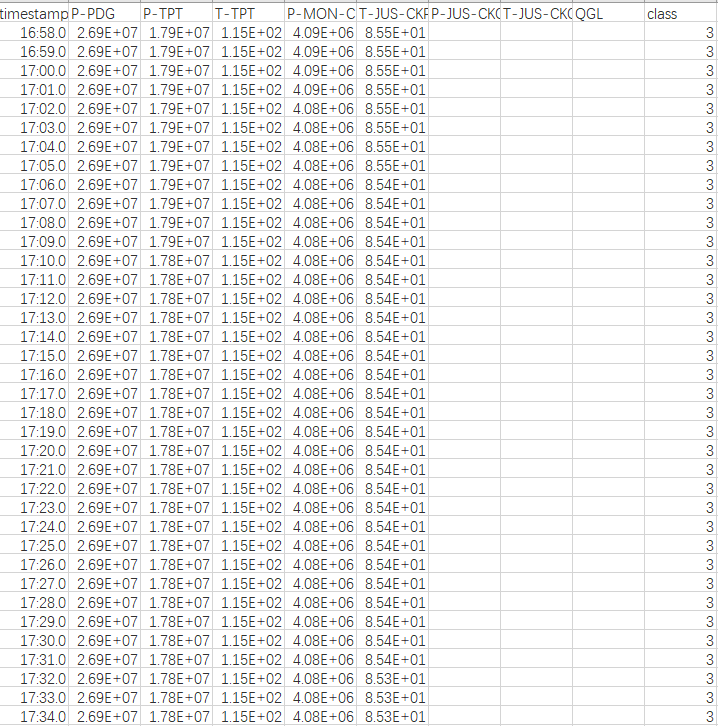
\includegraphics[height=9cm, width=12cm]{../resources/Before_Cleaning.png}
    \caption{进行清洗之前的数据}
\end{figure}
\begin{figure}[htbp]
    \centering
    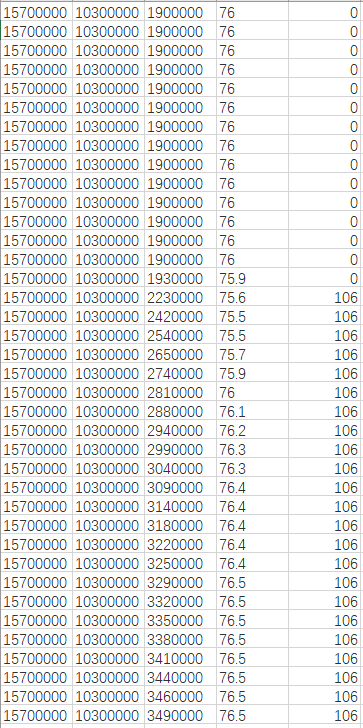
\includegraphics[height=10cm, width=6cm]{../resources/After_Cleaning.png}
    \caption{进行清洗之后的数据}
\end{figure}
\subsection{min-max 标准化}
在对数据进行清洗后,由于发现数据中存在较大的数据(假定为 $x \geq 10^8$),于是我在此进行了一次标准化,解决了由于数据过大而可能导致的错误。

此处我使用了 \texttt{Java-ML} 库中自带的 \texttt{NormalizeMidrange} 类,这是一个通过 min-max 标准化来对数据进行标准化的类。

min-max 标准化是将数据做以下运算:$$x^*=\dfrac{x - \min}{\max - \min}$$ 其中 $\max$ 为这组数据的最大值,$\min$ 为这组数据的最小值。

\texttt{NormalizeMidrange} 类有一个构造函数 \texttt{NormalizeMidrange(x, y)},表示标准化后数据将位于 $[2x-y, y]$ 的区间中。

\texttt{NormalizeMidrange} 类可以直接将 \texttt{Java-ML} 库中的 \texttt{Dataset} 类进行正则化,例如:
\begin{tcblisting}{listing engine=minted,boxrule=0.1mm,
    colback=blue!5!white,colframe=blue!75!black,
    listing only,left=5mm,enhanced,sharp corners=all,
    overlay={\begin{tcbclipinterior}\fill[red!20!blue!20!white] (frame.south west)
    rectangle ([xshift=5mm]frame.north west);\end{tcbclipinterior}},
    minted language=java,
    minted style=tango,
    minted options={fontsize=\small,breaklines,autogobble,linenos,numbersep=3mm,mathescape}}
Dataset d = FileHandler.loadDataset(new File("./resources/SIMULATED_00004.csv"), 4, ",");
NormalizeMidrange nmr = new NormalizeMidrange(1, 2);
nmr.build(d);
nmr.filter(d);
\end{tcblisting}

这表示通过 \texttt{nmr} 的标准化后,我们将数据集中的所有数据都放缩到了 $[0, 2]$ 这一区间。
\subsection{使用 Java-ML 库中自带的 KNN 算法}

在 \texttt{Java-ML} 库中,其提供了 \texttt{KNearestNeighbors} 和 \texttt{KDTreeKNN} 两个实现 KNN 的类,不同处在于第一个是比较暴力的基于原理实现,在数据量较大时时间消耗较高,
而第二个是基于 KD-Tree 的优化,在数据量较大时能较好地保证时间的消耗。

调用这两个类进行分类的过程是类似的,下面以 \texttt{KNearestNeighbors} 为例:
\begin{enumerate}
    \item 首先新建对象 \mintinline{java}{KNearestNeighbors knn = new KNearestNeighbors(k);},这里调用了含参构造函数 \texttt{KNearestNeighbors(int k)},其中的 \texttt{k}
 对应着 KNN 中的超参数 \texttt{k};
    \item 接着向对象中传入训练集 \mintinline{java}{knn.buildClassifier(train)},此处的数据集 \texttt{train} 被要求必须为 \texttt{Dataset} 类型,这是 \texttt{Java-ML} 库中
为数据集定义的类型;
    \item 对于测试集 \texttt{test} 中的每一行数据,我们可以通过一个 \texttt{for-in} 循环遍历,之后对每行数据进行分类并得到预测值:
    \begin{tcblisting}{listing engine=minted,boxrule=0.1mm,
        colback=blue!5!white,colframe=blue!75!black,
        listing only,left=5mm,enhanced,sharp corners=all,
        overlay={\begin{tcbclipinterior}\fill[red!20!blue!20!white] (frame.south west)
        rectangle ([xshift=5mm]frame.north west);\end{tcbclipinterior}},
        minted language=java,
        minted style=tango,
        minted options={fontsize=\small,breaklines,autogobble,linenos,numbersep=3mm,mathescape}}
for(Instance inst: test)
{
    Object classified = knn.classify(inst);
    if(classified.equals(inst.classValue())
        //correct, do sth
}
 \end{tcblisting}
    向 \texttt{classify} 函数中传入一条数据后,其会对数据进行分类,并返回一个 \texttt{Object} 类型的对象表示分类结果。如果分类结果与真实结果(即 \texttt{inst.classValue()})一致,
    表示分类正确,否则为分类错误。
\end{enumerate}

\subsection{手写 KNN 算法}

在本项目的仓库中,我是用的是自己基于原理手写的 KNN 算法,其大概分为如下几个部分:

\subsubsection{计算欧几里得距离}
\begin{tcblisting}{listing engine=minted,boxrule=0.1mm,
    colback=blue!5!white,colframe=blue!75!black,
    listing only,left=5mm,enhanced,sharp corners=all,
    overlay={\begin{tcbclipinterior}\fill[red!20!blue!20!white] (frame.south west)
    rectangle ([xshift=5mm]frame.north west);\end{tcbclipinterior}},
    minted language=java,
    minted style=tango,
    minted options={fontsize=\small,breaklines,autogobble,linenos,numbersep=3mm,mathescape}}
private double GetEuclidDistance(Instance x, Instance y)
{
	if(x.noAttributes() != y.noAttributes())
		throw new RuntimeException("Both instance should have the same number of values, Error!");
	double Dis = 0;
	for(int i = 0;i < x.noAttributes();i++)
	{
		if(!Double.isNaN(x.value(i)) && !Double.isNaN(y.value(i)))
				Dis += (y.value(i) - x.value(i)) * (y.value(i) - x.value(i));
	}
	return Math.sqrt(Dis);		
}
\end{tcblisting}

在这个函数中,首先需要比较数据 $x$ 和数据 $y$ 的维数是否相同(即 \texttt{x.noAttributes() != y.noAttributes()} 是否成立),如果维数不相同的话,计算其 Euclid 距离是没有意义的,
此时直接抛出一个运行错误;如果维数相同,便可以继续计算他们之间的 Euclid 距离。

\subsubsection{寻找前 K 个最近邻居}
\begin{tcblisting}{listing engine=minted,boxrule=0.1mm,
    colback=blue!5!white,colframe=blue!75!black,
    listing only,left=5mm,enhanced,sharp corners=all,
    overlay={\begin{tcbclipinterior}\fill[red!20!blue!20!white] (frame.south west)
    rectangle ([xshift=5mm]frame.north west);\end{tcbclipinterior}},
    minted language=java,
    minted style=tango,
    minted options={fontsize=\small,breaklines,autogobble,linenos,numbersep=3mm,mathescape}}
private Set<Instance> kNearest(Instance inst)
{
	Set<Instance> ExpectedInstance = new HashSet<>();
	HashMap<Double, Instance> dis = new HashMap<>();
	for(Instance Candidate: d)
	{
		double dist = GetEuclidDistance(Candidate, inst);
		dis.put(dist, Candidate);
	}
	TreeMap<Double, Instance> SortedDis = new TreeMap<>();
	SortedDis.putAll(dis);
	int count = 0;
	for(Map.Entry<Double, Instance> e: SortedDis.entrySet())
	{
		if(!ExpectedInstance.contains(e.getValue()))
		{
			ExpectedInstance.add(e.getValue());
			count++;
			if(count == k)
				break;
		}
	}
	return ExpectedInstance;
}
\end{tcblisting}

在这个函数中,我通过一个 \texttt{Set} 来保证取出的 $k$ 个数据都是互异的,
通过 \texttt{TreeMap} 和 \texttt{HashMap} 的配合达到为所有数据点以距离升序的要求排序的目的。
最后通过一个 \texttt{for-in} 循环,取出距离测试数据最近的 $k$ 个数据并放入集合 \texttt{ExpectedInstance} 中并作为这个函数的返回值。

\subsubsection{找到出现次数最多的标签}
\begin{tcblisting}{listing engine=minted,boxrule=0.1mm,
    colback=blue!5!white,colframe=blue!75!black,
    listing only,left=5mm,enhanced,sharp corners=all,
    overlay={\begin{tcbclipinterior}\fill[red!20!blue!20!white] (frame.south west)
    rectangle ([xshift=5mm]frame.north west);\end{tcbclipinterior}},
    minted language=java,
    minted style=tango,
    minted options={fontsize=\small,breaklines,autogobble,linenos,numbersep=3mm,mathescape}}
public Object classify(Instance inst)
{
	if(d == null)
		throw new RuntimeException("Training dataset is null");
	Set<Instance> NearNeighbors = kNearest(inst);
	Object[] ExpectedClass = new Object[k];
	int index = 0;
	for(Instance i: NearNeighbors)
		ExpectedClass[index++] = i.classValue();
	HashMap<Object, Integer> map = new HashMap<>();
	for(Object i: ExpectedClass)
	{
		if(map.containsKey(i))
		{
			int tmp = map.get(i);
			map.put(i, tmp + 1);
		}
		else
			map.put(i, 1);
	}
	Collection<Integer> count = map.values();
	int Maxcount = Collections.max(count);
	for(Map.Entry<Object, Integer> e: map.entrySet())
		if(Maxcount == e.getValue())
			return e.getKey();
	return null;
}
\end{tcblisting}

在这个函数中,首先需要判断训练集 \texttt{d} 是否为空,如果训练集为空的话对测试数据分类是没有意义的,于是直接抛出一个运行错误;如果不为空时,
首先会通过调用 \texttt{kNearest} 函数找到距离测试数据最近的前 $k$ 个数据,再将它们的分类标签记录在数组 \texttt{ExpectedClass} 中。下面通过一个 \texttt{HashMap} 和 \texttt{Collection}
 找到了这些分类标签中出现次数最多的一个标签,并返回其标签值。

\subsection{使用 Java-ML 库中自带的朴素贝叶斯算法}

朴素贝叶斯算法的代码与“使用 Java-ML 库中自带的 KNN 算法”部分基本一致,不同的是在新建对象时:
\mintinline{java}{NaiveBayesClassifier nbc = new NaiveBayesClassifier(true, true, false);} 其中调用了一个构造函数 \texttt{NaiveBayesClassifier(bool lap, bool log, bool sparse)},
第一个参数 \texttt{lap} 表示是否使用拉普拉斯平滑,第二个参数 \texttt{log} 表示是否使用对数以防止因为计算机精度的原因而将结果近似为 0,第三个参数 \texttt{sparse} 表示数据集是否为稀疏的。

此处我将 \texttt{lap} 和 \texttt{log} 设为 \texttt{true},而将 \texttt{sparse} 设为 \texttt{false}。

\subsection{分类结果的可视化}

首先,在两个算法的测试代码中,我均加入了文件输出,将真实标签输出至 \texttt{Real$\_$Ans.csv} 中,预测标签输出至 \texttt{Predicted$\_$Ans.csv} 中:

\begin{tcblisting}{listing engine=minted,boxrule=0.1mm,
    colback=blue!5!white,colframe=blue!75!black,
    listing only,left=5mm,enhanced,sharp corners=all,
    overlay={\begin{tcbclipinterior}\fill[red!20!blue!20!white] (frame.south west)
    rectangle ([xshift=5mm]frame.north west);\end{tcbclipinterior}},
    minted language=java,
    minted style=tango,
    minted options={fontsize=\small,breaklines,autogobble,linenos,numbersep=3mm,mathescape}}
FileWriter fw = new FileWriter("./Real_Ans.csv");
fw.write("Real_index,Real_class\n");
for(int i = 0;i < sigma;i++)
{
    Instance inst = test.instance(ind[i]);
    fw.write(i + "," + inst.classValue() + "\n");
}
fw.close();
fw = new FileWriter("./Predicted_Ans.csv");
fw.write("Predicted_index,Predicted_class\n");
for(int i = 0;i < sigma;i++)
{
    Instance inst = test.instance(ind[i]);
    fw.write(i + "," + knn.classify(inst) + "\n");
}
fw.close();
\end{tcblisting}

之后,我使用了 \texttt{Python} 进行了可视化:

\begin{tcblisting}{listing engine=minted,boxrule=0.1mm,
    colback=blue!5!white,colframe=blue!75!black,
    listing only,left=5mm,enhanced,sharp corners=all,
    overlay={\begin{tcbclipinterior}\fill[red!20!blue!20!white] (frame.south west)
    rectangle ([xshift=5mm]frame.north west);\end{tcbclipinterior}},
    minted language=python,
    minted style=tango,
    minted options={fontsize=\small,breaklines,autogobble,linenos,numbersep=3mm,mathescape}}
import pandas as pd
import matplotlib.pyplot as plt
df = pd.read_csv('./Real_Ans.csv')
df1 = pd.read_csv('./Predicted_Ans.csv')
plt.scatter(df['Real_index'], df['Real_class'], 15, 'red')
plt.scatter(df1['Predicted_index'], df1['Predicted_class'], 15, 'black')
\end{tcblisting}

其中调用了 \texttt{pandas} 库进行数据的读入,调用 \texttt{pyplot} 库画出一个散点图,横轴为测试点的数据编号,纵轴为测试点的标签值。其中可视化程序会将真实标签对应的点标为红色,
预测标签对应的点标为黑色。如果预测结果与实际结果一致,则红色点与黑色点应当重合,由于黑色点是在红色点之后被画出的,重合时应当显示为黑色;而当预测结果与实际结果不一致时,两种颜色的点不会重合,
此时在同一个 $x$ 坐标下应当看到一个黑色的点和一个红色的点,分别表示预测错误的结果和实际的结果。

\begin{figure}[htbp]
    \centering
    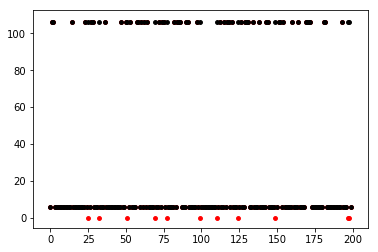
\includegraphics{./output.png}
    \caption{可视化结果}
\end{figure}

\appendix

\nocite{*}
\printbibliography[heading=bibintoc, title=\ebibname]
\end{document}